\chapter{Methodik}

\section{Eyetracking}

In dieser Studie wurde die Methode des Eyetrackings benutzt um die Blickbewegungen der Probanden auf dem Bildschirm fest zu halten. Im folgenden wird kurz die Einrichtung und die Funktionsweise eines Eyetracking Monitors beschrieben. 

Geräte, welche Blickbewegungen aufzeichnen können unterscheiden sich in zwei grundlegende Kathegorien:
    \begin{itemize}
        \item die eine Aufzeichnung über eine Brille erstellen
        \item die eine Kamera unterhalb des Bildschirms verwenden
    \end{itemize}


In diesem Versuchsaufbau wurde die 2. Variante gewählt. Hierbei ist es sehr wichtig, dass der Proband auf der richtigen Höhe sitzt und einen ungehinderten Blick (keine Brille) auf den Bildschirm hat. Ebenso wichtig ist, dass der Proband seinen Kopf gerade hält und nur die Augen bewegt, bei einer übermäßigen Bewegung des Kopfes werden die aufgezeichneten Daten verfälscht. Bevor mit der eigentlichen Studie begonnen werden kann, muss die Kamera kalibriert werden, hierfür soll der Versuchsteilnehmer einem Punkt am Bildschirm folgen um eine richtige Einstellung des Gerätes hervorzurufen. 

Der Versuchsaufbau ist wie in der Abbildung Versuchsaufbau beschrieben, dass der Proband (P) vor dem Bildschirm mit Kamera sitzt und der Versuchsleiter (V) auf der anderen Seite des Bildschirms. Die Kamera, welche die Blickbewegungen des Probanden aufzeichnet sitzt unter dem Anzeigebildschirm. Dieser Aufbau wurde gewählt, damit der Proband einfach ``weiter'' oder das Ergebnis einer Aufgabe sagen kann ohne den Blick vom Anzeigebildschirm zu lösen. Bei einer der Verwendung einer Tastatur, würde der Proband jedes mal wenn er auf sie schaut, die Kalibrierung des Eyetrackinggerätes verändert und somit die Daten verfälschen. 

\begin{figure}[!ht]
\noindent\hspace{0.5mm}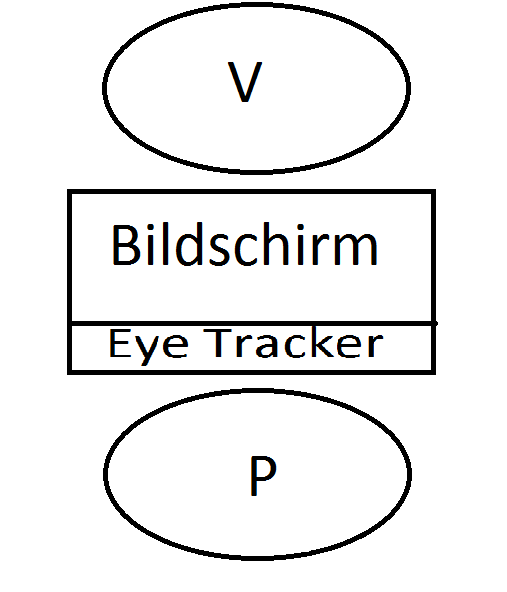
\includegraphics[width=8cm]{./Ressourcen/Versuchsaufbau.png}
\caption{Versuchsaufbau}
\end{figure}

\section{Begriffserklärung und Instrumentenbeschreibung}
Um diese Studie nachzuvollziehen werden im folgenden Teil einige Begriffe erklärt und angegeben wie die Daten ausgewertet wurden. 

Beginnend mit dem Begriff Fixationen auf ein bestimmtes Objekt ist in dieser Studie ein messbares innehalten des Probanden auf einer bestimmten Stelle des Bildschirms gemeint.``Diese Zeitdauer beträgt typischerweise 100 bis 200ms\cite{EyetrackingFixation} .''

Somit sind die Fixationen bei einer Auswertung von Eyetrackinguntersuchungen immer in drei Teile unterteilt:
    \begin{itemize}
        \item Die Koordinaten der einzelnen Fixation, meist aufgeteilt in einen x und einen y Wert.(Horizontal, Vertikal)
        \item Die Dauer der jeweiligen Fixation
        \item Die zeitliche Reihenfolge der Fixation
    \end{itemize}


Durch AOI`s (``Area of Interrest'') kann der für den Probanden sichtbare Bereich des Bildschirms in Abschnitte unterteilt werden, welche für die Auswertung relevant sind. In vorliegender Studie wurden auf der ersten Seite AOIs über die Textabschnitte, sowie über die Graphiken legt um die Fixationen auf diesem Bereich feststellen zu können. Ebenso wurde in den letzten Bereich eine AOI gelegt um das Unterscheiden von dem ersten zum zweiten Durchgang zu ermitteln (mehr dazu im Teil eigene Einteilung).

Eine Heatmap ist eine Darstellung des Bildschirms, in der die Benutzerfixationen anhand von ihrer Häufigkeit und Dauer eingefärbt werden. Hierbei können Zonen, welche vom Benutzer intensiv Betrachtet werden schnell veranschaulicht werden.

Diese Daten wurden mit Hilfe des Eyetrackingapperates RED 500 festgehalten und konnten in unter Verwendung des Programms IViewx unterteilt werden. Somit konnte die Anzahl der Fixationen in einem Bereich ausgewertet werden. Diese Daten wurde verwendet um die Gruppeneinteilung im folgenden Verlauf der Arbeit vorzunehmen.

Nach der Einteilung der Gruppen wurden zum einen Varianzanalysen zu den gegebenen Forschungsfragen angestellt. Die Auswertung erfolgte über einen einfaktorielle ANOVA um signifikante Unterschiede in den Gruppen oder unter den Bildern feststellen zu können. Zum anderen wurden die Mittelwerte berechnet und verglichen. Diese Auswertungen sind im Teil Ergebnis festgehalten.

\section{Ablauf der Studie}

Auf der ersten Folie wurde den Versuchsteilnehmern ein Beweis von Teilbarkeit  von 3 oder 5 aufeinander folgender Zahlen anhand eines Heuristischem Lösungsbeispiels veranschaulicht. Hierbei wurde gezeigt, dass 3 aufeinander folgende Zahlen z.B 3,4,5 in der Summe, also in unserem Beispiel 12, wieder durch die Anzahl der aufeinander folgenden Zahlen teilbar mit Ganzzahligem Ergebnis ist. Somit kann in unserem Beispiel die 12 durch 3 geteilt werden, ohne einen Rest zu haben.
Analog funktioniert es bei jeder ungeraden Anzahl an aufeinander folgender Natürlicher Zahlen. Die erste Folie unterteilt sich in Heuristiken, welche den allgemeinen Lösungsweg des Beweises aufzeigen soll und in Inhalt, welcher von textueller und bildlicher Form sein kann. In bildlicher Form ist zum einen ein Anfangsbeispiel, bei dem die Hypothese bei unterschiedlichen Zahlen überprüft wird. Zum anderen eine Möglichkeit, wie man durch Sortierung den Sachverhalt besser zu veranschaulichen. Im textueller Form wurden die Überlegungen festgehalten.

Darauf folgend wurden den Probanden 9 mathematische Aufgaben gestellt, welche sie mit Hilfe einer multiple choice Antwortmöglichkeit beantworten sollten. Ein Beispiel für eine Aufgabe ist:

\begin{figure}[H]
\noindent\hspace{0.5mm}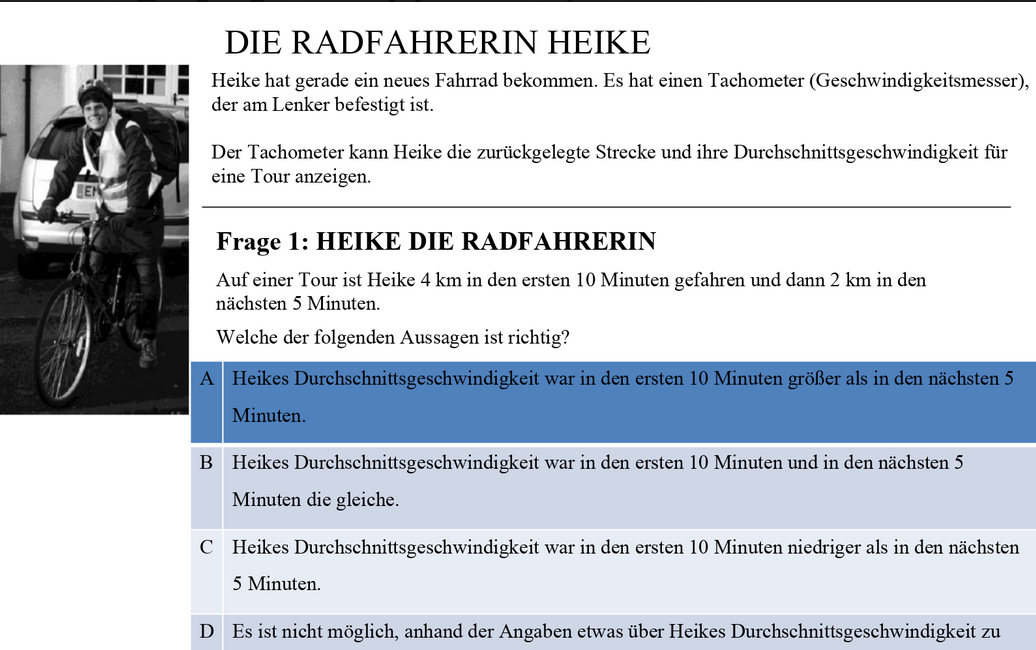
\includegraphics[width=17cm]{./Ressourcen/Radfahrerin.png}
\caption{Radfahrerin}
\end{figure}

\section{Eigene Aufgabe-Bildeinteilung}

In dieser Studie wurden die zugegebenen Bilder und Graphiken wie folgt unterteilt:

In ersten beiden Aufgabestellungen geht es um eine Radfahrerin, wobei lediglich ein Bild dieser Radfahrerin abgebildet ist. Dieses Bild trägt nicht zur Veranschaulichung oder Unterstützung der Versuchsperson bei und ist somit dekorativ. 


In der nächsten Aufgabenstellung ist ein Graph über die Geschwindigkeit eines Rennfahrers in Abhängigkeit vom Weg zu sehen. Dieser Graph muss verwendet werden, um die Aufgabenstellung zu bearbeiten und ist somit essenziell. 


In der darauf folgenden geschilderten Problematik sind 2 Graphiken, welche Teile eines Zufallsexperimentes darstellen verwendet. Hierbei müssen die Felder des Glücksrades und die Verteilung der Kugeln betrachtet werden um die Aufgabenstellung lösen zu können und somit sind die Graphiken auch essenziell.


Die nächsten beiden Aufgaben handeln vom Bergsteigen, hierbei ist lediglich ein Berg als Bild gegeben, welcher aber für die Bearbeitung der Aufgabe aber nicht nützlich ist, somit ist das Bild dekorativ. 


Im Anschluss wird noch eine Aufgabe im Themenbereich des Autofahrens gegeben. Dabei wurde wiederum ein Graph verwendet, der die Geschwindigkeit und die Zeit der Autofahrerin in Relation setzt. Diese Graphik ist wiederum essenziell für die Bearbeitung der Aufgabe. 


In den letzten beiden Aufgabestellungen wurde sowohl eine Tabelle, welche essenziell für die Bearbeitung ist, als auch ein einfaches Bild von einem Auto, welches eher dekorativen Charakter hat, verwendet. Da hierbei eine Mischung von Bildtypen verwendet wurde werden diese beiden Aufgaben in der weiteren Bearbeitung nicht weiter betrachtet. 

Somit kommen in dieser Bildunterteilung lediglich drei essenzielle und vier dekorative Bilder vor und keine repräsentativen Bilder. Somit sollte der Unterschied zwischen hilfreichen und nicht hilfreichen Bildern besser sichtbar sein.


\section{Eigene Gruppeneinteilung}

Aus den oben genannten Lerntypen wurden drei Gruppierungen gebildet: \gls{Gr1} der Unsichere, \gls{Gr2} der Problemlöser, \gls{Gr3} der Textuelle. Die gegebenen 39 Probanden wurden in die vorliegenden Typen unterteilt nach folgender Tabelle. 22 der Versuchsteilnehmer konnten in jeweils eine der Gruppierungen unterteilt werden. Bei den restlichen 17 war dies leider nicht möglich. Das erstmalige lesen des Textes dauerte dauerte im Schnitt über alle Probanden 110,4 Sekunden. Diese Dauer konnte ermittelt werden, indem in einer AOI am Ende des Textes Fixationen festgestellt wurden. Sobald also ein Proband in dieses Feld geblickt, ist der erste Durchgang des Lesevorgangs beendet und der Zweite beginnt, welcher andauert, bis der Proband auf die nächste Folie wechselt. Diese Einteilung konnte anhand von Messungen der Zeit und der Reihenfolge der Fixationen belegt werden. 


Die Probanden wiesen in der Allgemeinheit noch folgenden Werte im Durchschnitt auf:
    \begin{itemize}
        \item Dauer des Zweiten Durchgangs: 72,6 Sekungen 
        \item Fixationen auf die Bildbereiche im zweiten Durchgang: 75,2
        \item Fixationen auf die Textbereiche im zweiten Durchgang: 71,1
    \end{itemize}

Die Probanden wurden auf die genannten Merkmale untersucht und in die passen den Gruppen anhand dieser Einteilung zugeordnet.
\section*{Einteilungsschema}

\begin{table}[!h]
\hspace{-5pt}
\begin{tabularx}{\textwidth + 5pt}{| @{\hspace{3pt}} M || @{\hspace{3pt}} M  | @{\hspace{3pt}} M  | @{\hspace{3pt}} M |}
\hline
\textbf{Ausprägungen} & \textbf{Typ Unsicher (Gr1.)} & \textbf{Typ Problemlöser (Gr2.)} & \textbf{Typ Textuell (Gr3.)}\\
\hline
\hline
Dauer 1. Durchgang          & (+) & 0 & 0\\
\hline
Dauer 2. Durchgang          & ++ & 0 & (+)\\
\hline
Textfixationen 2. Durchgang & + & 0 & +\\
\hline
Bildfixationen 2. Durchgang & + & + & 0\\
\hline
\end{tabularx}
\caption{Ausprägungen}
\end{table}



\section{Schwierigkeiten bei der Erfassung}

Bei der Erfassung der Punkte einer Aufgabe ist lediglich ein Punkt vergeben worden, wenn die Aufgabe richtig gelöst wurde. Kein Punkt ist vergeben worden, wenn die Lösung nicht stimmt, somit wurden keine Teilpunkte vergeben. Wenn ein Proband die Aufgabe zu Teilen richtig löst, anschließend aber sich einen Denkfehler erlaubt bekommt er dennoch 0 Punkte auf die Aufgabe. Hierbei findet somit eine ergebnisorientierte- und keine lösungswegorientierte Auswertung der Aufgaben statt, welche die Fähigkeiten der Probanden schlechter abbildet als sie eigentlich wären.

Zusätzlich wurden Multiplechoicefrage Antwortmöglichkeiten gegeben. Diese beiden Voraussetzungen erzeugen eine Unschärfe der Antwort des Probanden. Eine Verbesserung der Leistung des Probanden wird durch die vierfache Antwortmöglichkeit der Aufgaben gegeben, da der Proband durch raten der Richtigen Lösung mit einer Wahrscheinlichkeit von 1/4 oder 25 Prozent richtig liegt. Dies hat zur Folge, dass die Fähigkeiten der Probanden besser abgebildet werden als sie eigentlich wären.  

Ebenso war es für die Probanden nicht möglich sich Aufgabenteile zu markieren, oder sich Notizen oder Rechnungen auf Papier nebenbei zu machen, dies hätte Kalibrierungsprobleme des Eye Tracking Automaten hervorrufen können. Dies könnte man meinen, sollte sich auch negativ aus die Auswertung der Aufgaben auswirken, jedoch haben Schukajlow und Leiss (2011) gezeigt, dass ``(b)ezüglich der selbstberichteten Strategienutzung und der mathematischen Modellierungsleistungen der Lernenden konnten keine signifikanten Korrelationen festgestellt werden\cite{schukajlow2011selbstberichtete}.'' Somit dieser Punkt nicht mit Sicherheit als ein Nachteil des Probanden gewertet werden. 

Die Einschränkungen der Ergebnisauswahl und der nur ergebnisorientierten Auswertungsansatz wurden so gewählt, weil sie die Auswertung der Studie deutlich vereinfacht haben.  Zusätzlich könnten sich auch beide Effekte im besten Fall aufgehoben haben.  

\section{Forschungsfrage}

Texte werden von den Versuchsteilnehmern unterschiedlich bearbeitet, hierbei liegen unterschiedliche Teilbereiche in textueller oder in bildlicher Form im Fokus. Häufig ist das lesen beim ersten Mal ein relativ linearer Vorgang, von links nach rechts und dann von oben nach unten gelesen. Nach dem ersten Durchgang unterscheiden Sich die Probanden und einzelne Teilbereiche des Textes werden einer weiteren Betrachtung unterzogen. Dies führt uns zu der Frage:
(1) Kann man die Probanden anhand ihrer Augenbewegungen in Gruppen unterteilen, (2) ob die Unterteilung Aufschlüsse die Leistungsfähigkeit innerhalb der Gruppe gibt?

Ein weitere Teil der Studie ist, das Ergebnis von Matthias Böckmann und Stanislaw Schukajlow (2018) in unserer Studie zu verifizieren (3), indem die unterteilten Aufgaben und die Gesamtpunktzahl der jeweiligen Aufgabe betrachtet wird. Somit wird untersucht ob ein direkter Zusammenhang zwischen der Lösung der Aufgabe und dem Typ des verwendeten Bildes besteht. Zuletzt wird noch untersucht, ob bestimmte Aufgabentypen für einzelne Probandengruppen positive oder auch negative Auswirkungen haben (4).